\documentclass[ignorenonframetext,aspectratio=169]{beamer}
\setbeamertemplate{caption}[numbered]
\setbeamertemplate{caption label separator}{: }
\setbeamercolor{caption name}{fg=normal text.fg}
\beamertemplatenavigationsymbolsempty
\usepackage{lmodern}
\usepackage{amssymb,amsmath}
\usepackage{ifxetex,ifluatex}
\usepackage{fixltx2e} % provides \textsubscript
\ifnum 0\ifxetex 1\fi\ifluatex 1\fi=0 % if pdftex
  \usepackage[T1]{fontenc}
  \usepackage[utf8]{inputenc}
\else % if luatex or xelatex
  \ifxetex
    \usepackage{mathspec}
  \else
    \usepackage{fontspec}
  \fi
  \defaultfontfeatures{Ligatures=TeX,Scale=MatchLowercase}
\fi
% use upquote if available, for straight quotes in verbatim environments
\IfFileExists{upquote.sty}{\usepackage{upquote}}{}
% use microtype if available
\IfFileExists{microtype.sty}{%
\usepackage{microtype}
\UseMicrotypeSet[protrusion]{basicmath} % disable protrusion for tt fonts
}{}
\newif\ifbibliography
\usepackage{color}
\usepackage{fancyvrb}
\newcommand{\VerbBar}{|}
\newcommand{\VERB}{\Verb[commandchars=\\\{\}]}
\DefineVerbatimEnvironment{Highlighting}{Verbatim}{commandchars=\\\{\}}
% Add ',fontsize=\small' for more characters per line
\newenvironment{Shaded}{}{}
\newcommand{\KeywordTok}[1]{\textcolor[rgb]{0.00,0.44,0.13}{\textbf{{#1}}}}
\newcommand{\DataTypeTok}[1]{\textcolor[rgb]{0.56,0.13,0.00}{{#1}}}
\newcommand{\DecValTok}[1]{\textcolor[rgb]{0.25,0.63,0.44}{{#1}}}
\newcommand{\BaseNTok}[1]{\textcolor[rgb]{0.25,0.63,0.44}{{#1}}}
\newcommand{\FloatTok}[1]{\textcolor[rgb]{0.25,0.63,0.44}{{#1}}}
\newcommand{\ConstantTok}[1]{\textcolor[rgb]{0.53,0.00,0.00}{{#1}}}
\newcommand{\CharTok}[1]{\textcolor[rgb]{0.25,0.44,0.63}{{#1}}}
\newcommand{\SpecialCharTok}[1]{\textcolor[rgb]{0.25,0.44,0.63}{{#1}}}
\newcommand{\StringTok}[1]{\textcolor[rgb]{0.25,0.44,0.63}{{#1}}}
\newcommand{\VerbatimStringTok}[1]{\textcolor[rgb]{0.25,0.44,0.63}{{#1}}}
\newcommand{\SpecialStringTok}[1]{\textcolor[rgb]{0.73,0.40,0.53}{{#1}}}
\newcommand{\ImportTok}[1]{{#1}}
\newcommand{\CommentTok}[1]{\textcolor[rgb]{0.38,0.63,0.69}{\textit{{#1}}}}
\newcommand{\DocumentationTok}[1]{\textcolor[rgb]{0.73,0.13,0.13}{\textit{{#1}}}}
\newcommand{\AnnotationTok}[1]{\textcolor[rgb]{0.38,0.63,0.69}{\textbf{\textit{{#1}}}}}
\newcommand{\CommentVarTok}[1]{\textcolor[rgb]{0.38,0.63,0.69}{\textbf{\textit{{#1}}}}}
\newcommand{\OtherTok}[1]{\textcolor[rgb]{0.00,0.44,0.13}{{#1}}}
\newcommand{\FunctionTok}[1]{\textcolor[rgb]{0.02,0.16,0.49}{{#1}}}
\newcommand{\VariableTok}[1]{\textcolor[rgb]{0.10,0.09,0.49}{{#1}}}
\newcommand{\ControlFlowTok}[1]{\textcolor[rgb]{0.00,0.44,0.13}{\textbf{{#1}}}}
\newcommand{\OperatorTok}[1]{\textcolor[rgb]{0.40,0.40,0.40}{{#1}}}
\newcommand{\BuiltInTok}[1]{{#1}}
\newcommand{\ExtensionTok}[1]{{#1}}
\newcommand{\PreprocessorTok}[1]{\textcolor[rgb]{0.74,0.48,0.00}{{#1}}}
\newcommand{\AttributeTok}[1]{\textcolor[rgb]{0.49,0.56,0.16}{{#1}}}
\newcommand{\RegionMarkerTok}[1]{{#1}}
\newcommand{\InformationTok}[1]{\textcolor[rgb]{0.38,0.63,0.69}{\textbf{\textit{{#1}}}}}
\newcommand{\WarningTok}[1]{\textcolor[rgb]{0.38,0.63,0.69}{\textbf{\textit{{#1}}}}}
\newcommand{\AlertTok}[1]{\textcolor[rgb]{1.00,0.00,0.00}{\textbf{{#1}}}}
\newcommand{\ErrorTok}[1]{\textcolor[rgb]{1.00,0.00,0.00}{\textbf{{#1}}}}
\newcommand{\NormalTok}[1]{{#1}}

\usepackage{graphicx,grffile}
\makeatletter
\def\maxwidth{\ifdim\Gin@nat@width>\linewidth\linewidth\else\Gin@nat@width\fi}
\def\maxheight{\ifdim\Gin@nat@height>\textheight0.8\textheight\else\Gin@nat@height\fi}
\makeatother

% Prevent slide breaks in the middle of a paragraph:
\widowpenalties 1 10000
\raggedbottom

\AtBeginPart{
  \let\insertpartnumber\relax
  \let\partname\relax
  \frame{\partpage}
}
\AtBeginSection{
  \ifbibliography
  \else
    \let\insertsectionnumber\relax
    \let\sectionname\relax
    \frame{\sectionpage}
  \fi
}
\AtBeginSubsection{
  \let\insertsubsectionnumber\relax
  \let\subsectionname\relax
  \frame{\subsectionpage}
}

\setlength{\parindent}{0pt}
\setlength{\parskip}{6pt plus 2pt minus 1pt}
\setlength{\emergencystretch}{3em}  % prevent overfull lines
\providecommand{\tightlist}{%
  \setlength{\itemsep}{0pt}\setlength{\parskip}{0pt}}
\setcounter{secnumdepth}{0}
\DeclareUnicodeCharacter{00A0}{~}
\DeclareUnicodeCharacter{03B4}{$\delta$}
\DeclareUnicodeCharacter{03B5}{$\varepsilon$}
\DeclareUnicodeCharacter{03C9}{$\omega$}
\DeclareUnicodeCharacter{2124}{\mathbb{Z}}
\DeclareUnicodeCharacter{2193}{$\downarrow$}
\DeclareUnicodeCharacter{2208}{$\in$}
\DeclareUnicodeCharacter{2209}{$\notin$}
\DeclareUnicodeCharacter{220B}{$\ni$}
\DeclareUnicodeCharacter{2227}{$\wedge$}
\DeclareUnicodeCharacter{2228}{$\vee$}
\DeclareUnicodeCharacter{2234}{$\therefore$}
\DeclareUnicodeCharacter{2264}{$\leq$}
\DeclareUnicodeCharacter{2265}{$\geq$}
\DeclareUnicodeCharacter{2605}{$\star$}
\DeclareUnicodeCharacter{1D53D}{\mathbb{F}}

% Scale images if necessary, so that they will not overflow the page
% margins by default, and it is still possible to overwrite the defaults
% using explicit options in \includegraphics[width, height, ...]{}
%\setkeys{Gin}{width=\maxwidth,height=\maxheight,keepaspectratio}
\newcommand{\includegraphicsscaled}[1]{
    \includegraphics[width=\maxwidth,height=\maxheight,keepaspectratio]{#1}
}

\usefonttheme[onlymath]{serif}
\hypersetup{breaklinks=true,colorlinks,linkcolor=,urlcolor=purple}
\setbeamertemplate{navigation symbols}{}
\setbeamercolor{footnote mark}{fg=gray}
\setbeamerfont{footnote}{size=\tiny}
\usepackage[normalem]{ulem}

\newcommand\greyuline{\bgroup\markoverwith
    {\textcolor{lightgray}{\rule[-0.5ex]{2pt}{0.4pt}}}\ULon}

\title{\bf Taming the C Monster}
\subtitle{\bf Haskell FFI Techniques}
\author{\bf Fraser Tweedale\\
    \texttt{@hackuador}}
\date{\bf May 22, 2018}

\setbeamertemplate{background}{
  \ifnum\thepage<2%
   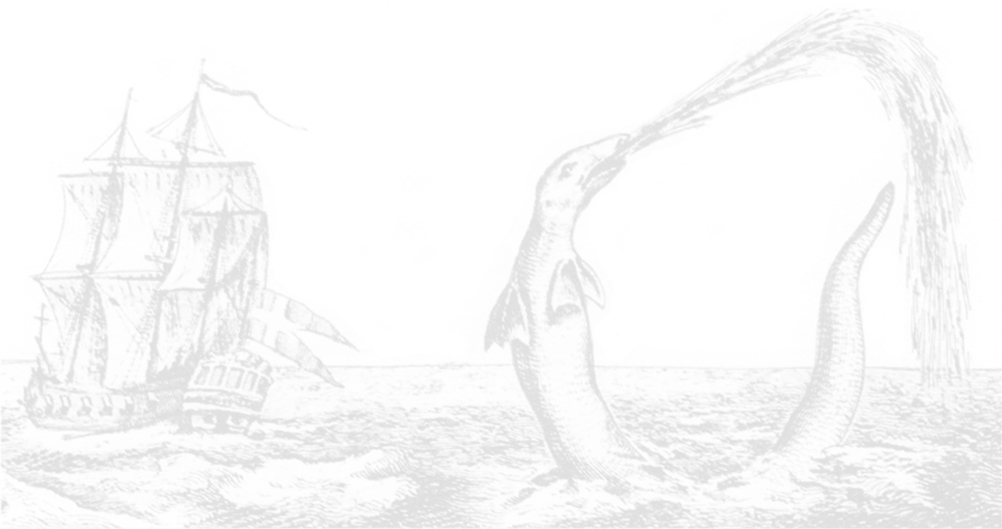
\includegraphics[height=\paperheight,width=\paperwidth]{Hans_Egede_sea_serpent_1734-light.jpg}
  \fi
}

\begin{document}

\begin{frame}
\titlepage
\end{frame}

\begin{frame}[plain]
\begin{center}
\includegraphicsscaled{mutt.png}
\end{center}
\end{frame}

\begin{frame}[plain]
\begin{center}
\includegraphicsscaled{notmuch.png}
\end{center}
\end{frame}

\begin{frame}[plain]
\begin{center}
\includegraphicsscaled{c-monster.jpg}
\end{center}
\end{frame}

\begin{frame}[plain]
\begin{center}
\includegraphicsscaled{sailor-attack.jpg}
\end{center}
\end{frame}

\begin{frame}[plain]
\begin{center}
\includegraphicsscaled{purebred.png}
\end{center}
\end{frame}

\section{FFI basics}\label{ffi-basics}

\begin{frame}{why FFI?}

\begin{itemize}
\tightlist
\item
  want to do \$THING in Haskell
\item
  there exists a C library for \$THING
\item
  interoperability / bug-compatibility
\item
  performance / timing-critical code
\end{itemize}

\end{frame}

\begin{frame}[fragile]{C FFI}

\begin{Shaded}
\begin{Highlighting}[]
\OtherTok{\{-# LANGUAGE ForeignFunctionInterface #-\}}

\KeywordTok{import} \DataTypeTok{Foreign.C.Types}

\KeywordTok{foreign import} \NormalTok{ccall} \StringTok{"math.h sin"}
\OtherTok{  c_sin ::} \DataTypeTok{CDouble} \OtherTok{->} \DataTypeTok{CDouble}

\OtherTok{main ::} \DataTypeTok{IO} \NormalTok{()}
\NormalTok{main }\FunctionTok{=} \NormalTok{print }\FunctionTok{$} \NormalTok{c_sin }\FloatTok{1.0}
\end{Highlighting}
\end{Shaded}

\end{frame}

\begin{frame}[fragile]{\tt hsc2hs}

\begin{itemize}
\tightlist
\item
  file extension: \texttt{.hsc}
\item
  part of GHC distribution
\item
  good support for marshalling structs
\end{itemize}

\end{frame}

\begin{frame}[fragile]{\tt c2hs}

\begin{itemize}
\tightlist
\item
  file extension: \texttt{.chs}
\item
  more features than \texttt{hsc2hs}
\item
  automatic generation of \texttt{foreign\ import} declarations
\end{itemize}

\begin{verbatim}
library
  ...
  build-tools:
    c2hs >= 0.19.1
\end{verbatim}

\end{frame}

\begin{frame}[fragile]{\texttt{c2hs} - example}

\begin{Shaded}
\begin{Highlighting}[]
...
  \NormalTok{result }\OtherTok{<-} \StringTok{\{#}\KeywordTok{call} \StringTok{notmuch_database_open #\}} \NormalTok{path \DecValTok{1} ptr}
  ...
\end{Highlighting}
\end{Shaded}

\end{frame}

\begin{frame}[fragile]{\texttt{c2hs} - example}

\begin{Shaded}
\begin{Highlighting}[]
...
  \NormalTok{result }\OtherTok{<-} \NormalTok{notmuch_database_open} \NormalTok{path \DecValTok{1} ptr}
  ...

\KeywordTok{foreign import} \NormalTok{ccall} \StringTok{"Notmuch/Binding.chs.h notmuch_database_open"}
  \NormalTok{notmuch_database_open}
\OtherTok{    ::} \DataTypeTok{CString} \OtherTok{->} \DataTypeTok{CInt} \OtherTok{->} \DataTypeTok{Ptr} \NormalTok{(}\DataTypeTok{Ptr} \DataTypeTok{Database}\NormalTok{) }\OtherTok{->} \DataTypeTok{IO} \DataTypeTok{CInt}
\end{Highlighting}
\end{Shaded}

\end{frame}

\begin{frame}[fragile]{\texttt{Foreign.Ptr}}

\begin{Shaded}
\begin{Highlighting}[]
\KeywordTok{data} \DataTypeTok{Ptr} \NormalTok{a}

\OtherTok{nullPtr ::} \DataTypeTok{Ptr} \NormalTok{a}

\OtherTok{plusPtr ::} \DataTypeTok{Ptr} \NormalTok{a }\OtherTok{->} \DataTypeTok{Int} \OtherTok{->} \DataTypeTok{Ptr} \NormalTok{b}

\OtherTok{castPtr ::} \DataTypeTok{Ptr} \NormalTok{a }\OtherTok{->} \DataTypeTok{Ptr} \NormalTok{b}
\end{Highlighting}
\end{Shaded}

\end{frame}

\begin{frame}[fragile]{\texttt{Foreign.ForeignPtr}}

\begin{Shaded}
\begin{Highlighting}[]
\KeywordTok{data} \DataTypeTok{ForeignPtr} \NormalTok{a}

\KeywordTok{type} \DataTypeTok{FinalizerPtr} \NormalTok{a }\FunctionTok{=} \DataTypeTok{FunPtr} \NormalTok{(}\DataTypeTok{Ptr} \NormalTok{a }\OtherTok{->} \DataTypeTok{IO} \NormalTok{())}

\OtherTok{newForeignPtr ::} \DataTypeTok{FinalizerPtr} \NormalTok{a }\OtherTok{->} \DataTypeTok{Ptr} \NormalTok{a }\OtherTok{->} \DataTypeTok{IO} \NormalTok{(}\DataTypeTok{ForeignPtr} \NormalTok{a)}

\OtherTok{withForeignPtr ::} \DataTypeTok{ForeignPtr} \NormalTok{a }\OtherTok{->} \NormalTok{(}\DataTypeTok{Ptr} \NormalTok{a }\OtherTok{->} \DataTypeTok{IO} \NormalTok{b) }\OtherTok{->} \DataTypeTok{IO} \NormalTok{b}
\end{Highlighting}
\end{Shaded}

\end{frame}

\begin{frame}[fragile]{\texttt{Foreign.C.String}}

\begin{Shaded}
\begin{Highlighting}[]
\KeywordTok{type} \DataTypeTok{CString} \FunctionTok{=} \DataTypeTok{Ptr} \DataTypeTok{CChar}

\OtherTok{peekCString ::} \DataTypeTok{CString} \OtherTok{->} \DataTypeTok{IO} \DataTypeTok{String}

\OtherTok{withCString ::} \DataTypeTok{String} \OtherTok{->} \NormalTok{(}\DataTypeTok{CString} \OtherTok{->} \DataTypeTok{IO} \NormalTok{a) }\OtherTok{->} \DataTypeTok{IO} \NormalTok{a}
\end{Highlighting}
\end{Shaded}

\end{frame}

\begin{frame}[fragile]{\texttt{Foreign.Storable}}

\begin{Shaded}
\begin{Highlighting}[]
\KeywordTok{class} \DataTypeTok{Storable} \NormalTok{a }\KeywordTok{where}
\OtherTok{  peek ::} \DataTypeTok{Ptr} \NormalTok{a }\OtherTok{->} \DataTypeTok{IO} \NormalTok{a}
  \OtherTok{...}

\KeywordTok{instance} \DataTypeTok{Storable} \NormalTok{(}\DataTypeTok{Ptr} \NormalTok{a)}


\CommentTok{-- Foreign.Marshal.Alloc}
\OtherTok{alloca ::} \DataTypeTok{Storable} \NormalTok{a }\OtherTok{=>} \NormalTok{(}\DataTypeTok{Ptr} \NormalTok{a }\OtherTok{->} \DataTypeTok{IO} \NormalTok{b) }\OtherTok{->} \DataTypeTok{IO} \NormalTok{b}
\end{Highlighting}
\end{Shaded}

\end{frame}

\section{C constructions and idioms}\label{c-constructions-and-idioms}

\begin{frame}[fragile]{enum types}

\begin{Shaded}
\begin{Highlighting}[]
\KeywordTok{typedef} \KeywordTok{enum} \NormalTok{_notmuch_status \{}
  \NormalTok{NOTMUCH_STATUS_SUCCESS = }\DecValTok{0}\NormalTok{,}
  \NormalTok{NOTMUCH_STATUS_OUT_OF_MEMORY,}
  \NormalTok{NOTMUCH_STATUS_READ_ONLY_DATABASE,}
  \NormalTok{NOTMUCH_STATUS_UNBALANCED_FREEZE_THAW,}
  \NormalTok{...}
\NormalTok{\} notmuch_status_t}
\end{Highlighting}
\end{Shaded}

\end{frame}

\begin{frame}[fragile]{enum types}

\begin{Shaded}
\begin{Highlighting}[]
\StringTok{\{#}\KeywordTok{enum} \StringTok{notmuch_status_t} as \DataTypeTok{Status} \StringTok{\{underscoreToCase\} \KeywordTok{deriving} (}\DataTypeTok{Eq}\StringTok{) #\}}
\end{Highlighting}
\end{Shaded}

\end{frame}

\begin{frame}[fragile]{enum types}

\begin{Shaded}
\begin{Highlighting}[]
\KeywordTok{data} \DataTypeTok{Status} \FunctionTok{=} \DataTypeTok{StatusSuccess}
            \FunctionTok{|} \DataTypeTok{StatusOutOfMemory}
            \FunctionTok{|} \DataTypeTok{StatusReadOnlyDatabase}
            \FunctionTok{|} \DataTypeTok{StatusUnbalancedFreezeThaw}
            \FunctionTok{...}
  \KeywordTok{deriving} \NormalTok{(}\DataTypeTok{Eq}\NormalTok{)}

\KeywordTok{instance} \DataTypeTok{Enum} \DataTypeTok{Status} \KeywordTok{where}
  \FunctionTok{...}
\end{Highlighting}
\end{Shaded}

\end{frame}

\begin{frame}[fragile]{opaque pointer types}

\begin{Shaded}
\begin{Highlighting}[]
\KeywordTok{typedef} \KeywordTok{struct} \NormalTok{_notmuch_database notmuch_database_t;}
\end{Highlighting}
\end{Shaded}

\end{frame}

\begin{frame}[fragile]{opaque pointer types}

\begin{Shaded}
\begin{Highlighting}[]
\StringTok{\{#}\KeywordTok{pointer}\StringTok{ *notmuch_database_t }\KeywordTok{as}\StringTok{ }\DataTypeTok{DatabaseHandle}\StringTok{ }\KeywordTok{foreign}\StringTok{ }\KeywordTok{newtype}\StringTok{ #\}}
\end{Highlighting}
\end{Shaded}

\end{frame}

\begin{frame}[fragile]{opaque pointer types}

\begin{Shaded}
\begin{Highlighting}[]
\KeywordTok{newtype} \DataTypeTok{DatabaseHandle} \FunctionTok{=} \DataTypeTok{DatabaseHandle} \NormalTok{(}\DataTypeTok{ForeignPtr} \DataTypeTok{DatabaseHandle}\NormalTok{)}

\NormalTok{withDatabaseHandle}
\OtherTok{  ::} \DataTypeTok{DatabaseHandle} \OtherTok{->} \NormalTok{(}\DataTypeTok{Ptr} \DataTypeTok{DatabaseHandle} \OtherTok{->} \DataTypeTok{IO} \NormalTok{b) }\OtherTok{->} \DataTypeTok{IO} \NormalTok{b}
\NormalTok{withDatabaseHandle (}\DataTypeTok{DatabaseHandle} \NormalTok{fptr) }\FunctionTok{=}
  \NormalTok{withForeignPtr fptr}
\end{Highlighting}
\end{Shaded}

\end{frame}

\begin{frame}[fragile]{double-pointer constructors}

\begin{Shaded}
\begin{Highlighting}[]
\NormalTok{notmuch_status_t}
\NormalTok{notmuch_database_open (}\DataTypeTok{const} \DataTypeTok{char} \NormalTok{*path,}
                       \NormalTok{notmuch_database_mode_t mode,}
                       \NormalTok{notmuch_database_t **database);}
\end{Highlighting}
\end{Shaded}

\end{frame}

\begin{frame}[fragile]{double-pointer constructors}

\begin{Shaded}
\begin{Highlighting}[]
\OtherTok{databaseOpen ::} \DataTypeTok{CString} \OtherTok{->} \DataTypeTok{IO} \NormalTok{(}\DataTypeTok{Either} \DataTypeTok{Status} \DataTypeTok{DatabaseHandle}\NormalTok{)}
\NormalTok{databaseOpen path }\FunctionTok{=}
  \NormalTok{\greyuline{alloca}} \FunctionTok{$} \NormalTok{\textbackslash{}ptr }\OtherTok{->} \KeywordTok{do}
    \NormalTok{result }\OtherTok{<-} \StringTok{\{#}\KeywordTok{call}\StringTok{ notmuch_database_open #\}} \NormalTok{path \DecValTok{1} ptr}
    \KeywordTok{case} \NormalTok{toEnum (fromIntegral result) }\KeywordTok{of}
      \DataTypeTok{StatusSuccess} \OtherTok{->}
        \DataTypeTok{Right} \FunctionTok{.} \DataTypeTok{DatabaseHandle} \FunctionTok{<$>} \NormalTok{(\greyuline{peek} ptr} \FunctionTok{>>=} \NormalTok{newForeignPtr_)}
      \NormalTok{e }\OtherTok{->}
        \NormalTok{pure (}\DataTypeTok{Left} \NormalTok{e)}
\end{Highlighting}
\end{Shaded}

\end{frame}

\begin{frame}[fragile]{iterator}

\begin{Shaded}
\begin{Highlighting}[]
\NormalTok{notmuch_tags_t *}
\NormalTok{notmuch_message_get_tags (notmuch_message_t *message);}

\NormalTok{notmuch_bool_t}
\NormalTok{notmuch_tags_valid (notmuch_tags_t *tags);}

\DataTypeTok{const} \DataTypeTok{char} \NormalTok{*}
\NormalTok{notmuch_tags_get (notmuch_tags_t *tags);}

\DataTypeTok{void}
\NormalTok{notmuch_tags_move_to_next (notmuch_tags_t *tags);}
\end{Highlighting}
\end{Shaded}

\end{frame}

%\begin{frame}[fragile]{iterator}

\begin{Shaded}
\begin{Highlighting}[]
\StringTok{\{#}\KeywordTok{pointer}\StringTok{ *notmuch_tags_t }\KeywordTok{as}\StringTok{ }\DataTypeTok{Tags}\StringTok{ }\KeywordTok{newtype}\StringTok{ #\}}
\end{Highlighting}
\end{Shaded}

\end{frame}

\begin{frame}[fragile]{iterator}

\begin{Shaded}
\begin{Highlighting}[]
\KeywordTok{newtype} \DataTypeTok{Tags} \FunctionTok{=} \DataTypeTok{Tags} \NormalTok{(}\DataTypeTok{Ptr} \DataTypeTok{Tags}\NormalTok{)}
\end{Highlighting}
\end{Shaded}

\end{frame}


\begin{frame}[fragile]{iterator}

\begin{Shaded}
\begin{Highlighting}[]
\OtherTok{tagsToList ::} \DataTypeTok{Tags} \OtherTok{->} \DataTypeTok{IO} \NormalTok{[}\DataTypeTok{String}\NormalTok{]}
\NormalTok{tagsToList (}\DataTypeTok{Tags} \NormalTok{ptr) }\FunctionTok{=} \NormalTok{go}
  \KeywordTok{where}
  \NormalTok{go} \FunctionTok{=} \NormalTok{\greyuline{test} ptr} \FunctionTok{>>=} \NormalTok{\textbackslash{}valid }\OtherTok{->} \KeywordTok{case} \NormalTok{valid }\KeywordTok{of}
    \DecValTok{0} \OtherTok{->} \NormalTok{pure []}
    \NormalTok{_ }\OtherTok{->} \NormalTok{(}\FunctionTok{:}\NormalTok{)}
          \FunctionTok{<$>} \NormalTok{(\greyuline{get} ptr} \FunctionTok{>>=} \NormalTok{\greyuline{mk}} \FunctionTok{>>=} \NormalTok{\textbackslash{}x} \OtherTok{->} \NormalTok{\greyuline{next} ptr} \FunctionTok{$>} \NormalTok{x)}
          \FunctionTok{<*>} \NormalTok{go}

  \NormalTok{test }\FunctionTok{=} \StringTok{\{#}\KeywordTok{call}\StringTok{ notmuch_tags_valid #\}}
  \NormalTok{get }\FunctionTok{=} \StringTok{\{#}\KeywordTok{call}\StringTok{ notmuch_tags_get #\}}
  \NormalTok{next }\FunctionTok{=} \StringTok{\{#}\KeywordTok{call}\StringTok{ notmuch_tags_move_to_next #\}}
  \NormalTok{mk }\FunctionTok{=} \NormalTok{peekCString}
\end{Highlighting}
\end{Shaded}

\end{frame}

\begin{frame}[fragile]{macros}

\begin{Shaded}
\begin{Highlighting}[]
\DataTypeTok{void} \NormalTok{*talloc_steal(}\DataTypeTok{const} \DataTypeTok{void} \NormalTok{*new_ctx, }\DataTypeTok{const} \DataTypeTok{void} \NormalTok{*ptr);}
\end{Highlighting}
\end{Shaded}

\end{frame}

\begin{frame}[fragile]{macros}

\begin{Shaded}
\begin{Highlighting}[]
\PreprocessorTok{#if (__GNUC__ >= 3)}
\PreprocessorTok{#define _TALLOC_TYPEOF(ptr) __typeof__(ptr)}
\PreprocessorTok{#define talloc_steal(ctx, ptr) (\{ \textbackslash{}}
\PreprocessorTok{  _TALLOC_TYPEOF(ptr) __talloc_steal_ret = (_TALLOC_TYPEOF(ptr)) \textbackslash{}}
\PreprocessorTok{    _talloc_steal_loc((ctx), (ptr), __location__); \textbackslash{}}
\PreprocessorTok{  __talloc_steal_ret; \})}
\PreprocessorTok{#else }\CommentTok{/* __GNUC__ >= 3 */}
\PreprocessorTok{#define _TALLOC_TYPEOF(ptr) void *}
\PreprocessorTok{#define talloc_steal(ctx, ptr) \textbackslash{}}
\PreprocessorTok{  (_TALLOC_TYPEOF(ptr)) _talloc_steal_loc((ctx), (ptr), __location__)}
\PreprocessorTok{#endif }\CommentTok{/* __GNUC__ >= 3 */}
\DataTypeTok{void} \NormalTok{*_talloc_steal_loc(}
  \DataTypeTok{const} \DataTypeTok{void} \NormalTok{*new_ctx, }\DataTypeTok{const} \DataTypeTok{void} \NormalTok{*ptr, }\DataTypeTok{const} \DataTypeTok{char} \NormalTok{*location);}
\end{Highlighting}
\end{Shaded}

\end{frame}

\begin{frame}[fragile]{macros}

Two options:

\begin{itemize}
\tightlist
\item
  bind to non-public API (e.g. \texttt{\_talloc\_steal\_loc})
\item
  write \emph{``c bits''}
\end{itemize}

\end{frame}

\begin{frame}[fragile]{external object lifecycles}

\begin{Shaded}
\begin{Highlighting}[]
\NormalTok{notmuch_query_t *}
\NormalTok{notmuch_query_create (notmuch_database_t *database,}
                      \DataTypeTok{const} \DataTypeTok{char} \NormalTok{*query_string);}

\DataTypeTok{void}
\NormalTok{notmuch_query_destroy (notmuch_query_t *query);}
\end{Highlighting}
\end{Shaded}

\end{frame}

\begin{frame}[fragile]{external object lifecycles}

\begin{Shaded}
\begin{Highlighting}[]
\OtherTok{query_create ::} \DataTypeTok{DatabaseHandle} \OtherTok{->} \DataTypeTok{String} \OtherTok{->} \DataTypeTok{IO} \NormalTok{(}\DataTypeTok{Query} \NormalTok{a)}
\NormalTok{query_create db s }\FunctionTok{=} \NormalTok{withCString s }\FunctionTok{$} \NormalTok{\textbackslash{}s' }\OtherTok{->}
  \NormalTok{withDatabaseHandle db }\FunctionTok{$} \NormalTok{\textbackslash{}db' }\OtherTok{->}
    \StringTok{\{#}\KeywordTok{call}\StringTok{ notmuch_query_create #\}} \NormalTok{db' s'}
      \FunctionTok{>>=} \NormalTok{fmap }\DataTypeTok{Query} \FunctionTok{.} \NormalTok{\greyuline{newForeignPtr query_destroy}}

\KeywordTok{foreign import} \NormalTok{ccall} \StringTok{"\greyuline{&}notmuch_query_destroy"}
  \OtherTok{query_destroy ::} \DataTypeTok{FinalizerPtr} \DataTypeTok{Query}
\end{Highlighting}
\end{Shaded}

\end{frame}

\begin{frame}[fragile]{external object lifecycles}

\begin{Shaded}
\begin{Highlighting}[]
\OtherTok{query_create ::} \DataTypeTok{DatabaseHandle} \OtherTok{->} \DataTypeTok{String} \OtherTok{->} \DataTypeTok{IO} \NormalTok{(}\DataTypeTok{Query} \NormalTok{a)}
\NormalTok{query_create db s }\FunctionTok{=} \NormalTok{withCString s }\FunctionTok{$} \NormalTok{\textbackslash{}s' }\OtherTok{->}
  \NormalTok{withDatabaseHandle db }\FunctionTok{$} \NormalTok{\textbackslash{}db' }\OtherTok{->}
    \StringTok{\{#}\KeywordTok{call}\StringTok{ notmuch_query_create #\}} \NormalTok{db' s'}
      \FunctionTok{>>=} \NormalTok{fmap }\DataTypeTok{Query} \FunctionTok{.} \NormalTok{\greyuline{newForeignPtr query_destroy}}

\KeywordTok{foreign import} \NormalTok{ccall} \StringTok{"\greyuline{&}notmuch_query_destroy"}
  \OtherTok{query_destroy ::} \DataTypeTok{FunPtr} \NormalTok{(}\DataTypeTok{Ptr} \DataTypeTok{Query} \OtherTok{->} \DataTypeTok{IO} \NormalTok{())}
\end{Highlighting}
\end{Shaded}

\end{frame}

\begin{frame}{external object lifecycles - beware}
\begin{itemize}
\tightlist
\item
  hidden references in derived objects
\item
  fancy allocators (e.g. \em{talloc})
\end{itemize}
\end{frame}

\section{API safety}\label{api-safety}

\begin{frame}[fragile]{read-only mode}

\begin{Shaded}
\begin{Highlighting}[]
\CommentTok{/* can return NOTMUCH_STATUS_READ_ONLY_DATABASE */}
\NormalTok{notmuch_status_t}
\NormalTok{notmuch_message_\greyuline{add_tag} (notmuch_message_t *message, }\DataTypeTok{const} \DataTypeTok{char} \NormalTok{*tag);}
\end{Highlighting}
\end{Shaded}

\end{frame}

\begin{frame}[fragile]{read-only mode}

\begin{Shaded}
\begin{Highlighting}[]
\StringTok{\{#}\KeywordTok{enum} \StringTok{notmuch_database_mode_t} as \DataTypeTok{DatabaseMode} \StringTok{\{underscoreToCase\} #\}}
\end{Highlighting}
\end{Shaded}

\end{frame}

\begin{frame}[fragile]{read-only mode}

\begin{Shaded}
\begin{Highlighting}[]
\KeywordTok{data} \DataTypeTok{DatabaseMode} \FunctionTok{=} \DataTypeTok{DatabaseModeReadOnly}
                  \FunctionTok{|} \DataTypeTok{DatabaseModeReadWrite}

\KeywordTok{instance} \DataTypeTok{Enum} \DataTypeTok{DatabaseMode} \KeywordTok{where}
  \FunctionTok{...}
\end{Highlighting}
\end{Shaded}

\end{frame}

\begin{frame}[fragile]{read-only mode}

\begin{Shaded}
\begin{Highlighting}[]
\OtherTok{\{-# LANGUAGE DataKinds #-\}}

\KeywordTok{newtype} \DataTypeTok{Database} \NormalTok{(}\greyuline{\OtherTok{a ::} \DataTypeTok{DatabaseMode}}\NormalTok{) }\FunctionTok{=} \DataTypeTok{Database} \DataTypeTok{DatabaseHandle}

\OtherTok{withDatabase ::} \DataTypeTok{Database} \NormalTok{a }\OtherTok{->} \NormalTok{(}\DataTypeTok{Ptr} \DataTypeTok{DatabaseHandle} \OtherTok{->} \DataTypeTok{IO} \NormalTok{b) }\OtherTok{->} \DataTypeTok{IO} \NormalTok{b}
\NormalTok{withDatabase (}\DataTypeTok{Database} \NormalTok{dbh) }\FunctionTok{=} \NormalTok{withDatabaseHandle dbh}

\KeywordTok{data} \DataTypeTok{Message} \NormalTok{(}\greyuline{\OtherTok{a ::} \DataTypeTok{DatabaseMode}}\NormalTok{)} \FunctionTok{=} \DataTypeTok{Message} \DataTypeTok{MessageHandle}
\end{Highlighting}
\end{Shaded}

\end{frame}

%\begin{frame}[fragile]{API safety - read-only mode}

\begin{Shaded}
\begin{Highlighting}[]
\KeywordTok{class} \DataTypeTok{Mode} \NormalTok{a }\KeywordTok{where}
\OtherTok{  getMode ::} \DataTypeTok{Proxy} \NormalTok{a }\OtherTok{->} \DataTypeTok{DatabaseMode}

\KeywordTok{instance} \DataTypeTok{Mode} \CharTok{'DatabaseModeReadOnly where}
  \NormalTok{getMode _ }\FunctionTok{=} \DataTypeTok{DatabaseModeReadOnly}

\KeywordTok{instance} \DataTypeTok{Mode} \CharTok{'DatabaseModeReadWrite where}
  \NormalTok{getMode _ }\FunctionTok{=} \DataTypeTok{DatabaseModeReadWrite}
\end{Highlighting}
\end{Shaded}

\end{frame}

\begin{frame}[fragile]{API safety - read-only mode}

\begin{Shaded}
\begin{Highlighting}[]
\OtherTok{\{-# LANGUAGE ScopedTypeVariables #-\}}

\NormalTok{databaseOpen}
\OtherTok{  ::} \NormalTok{forall a}\FunctionTok{.} \DataTypeTok{Mode} \NormalTok{a}
  \OtherTok{=>} \DataTypeTok{CString} \OtherTok{->} \DataTypeTok{IO} \NormalTok{(}\DataTypeTok{Either} \DataTypeTok{Status} \NormalTok{(}\DataTypeTok{Database} \NormalTok{a))}
\NormalTok{databaseOpen path }\FunctionTok{=}
  \KeywordTok{let}
    \NormalTok{mode }\FunctionTok{=} \NormalTok{getMode (}\DataTypeTok{Proxy}\OtherTok{ ::} \DataTypeTok{Proxy} \NormalTok{a)}
  \KeywordTok{in}
    \FunctionTok{...}
\end{Highlighting}
\end{Shaded}

\end{frame}


\begin{frame}[fragile]{read-only mode}

\begin{Shaded}
\begin{Highlighting}[]
\KeywordTok{type} \DataTypeTok{RW} \FunctionTok{=} \DataTypeTok{'DatabaseModeReadWrite}  \CommentTok{-- convenient alias}

\OtherTok{messageAddTag ::} \greyuline{\DataTypeTok{Message} \DataTypeTok{RW}} \OtherTok{->} \DataTypeTok{Tag} \OtherTok{->} \DataTypeTok{IO} \NormalTok{()}
\NormalTok{messageAddTag msg tag }\FunctionTok{=} \NormalTok{\greyuline{void}} \FunctionTok{$} \NormalTok{withMessage msg }\FunctionTok{$}
  \NormalTok{tagUseAsCString tag }\FunctionTok{.} \StringTok{\{#}\KeywordTok{call}\StringTok{ notmuch_message_add_tag #\}}
\end{Highlighting}
\end{Shaded}

\end{frame}

\begin{frame}[fragile]{locking}

\begin{Shaded}
\begin{Highlighting}[]
\CommentTok{/* can return NOTMUCH_STATUS_READ_ONLY_DATABASE */}
\NormalTok{notmuch_status_t}
\NormalTok{notmuch_message_freeze (notmuch_message_t *message);}

\CommentTok{/* can return NOTMUCH_STATUS_READ_ONLY_DATABASE}
\CommentTok{   or NOTMUCH_STATUS_UNBALANCED_FREEZE_THAW      */}
\NormalTok{notmuch_status_t}
\NormalTok{notmuch_message_thaw (notmuch_message_t *message);}
\end{Highlighting}
\end{Shaded}

\end{frame}

\begin{frame}[fragile]{locking}

\begin{Shaded}
\begin{Highlighting}[]
\OtherTok{\{-# LANGUAGE DataKinds #-\}}
\OtherTok{\{-# LANGUAGE TypeFamilies #-\}}
\OtherTok{\{-# LANGUAGE TypeOperators #-\}}

\KeywordTok{import }\DataTypeTok{GHC.TypeLits}

\KeywordTok{data} \DataTypeTok{Message} \NormalTok{(}\greyuline{\OtherTok{n ::} \DataTypeTok{Nat}}\NormalTok{) (}\OtherTok{a ::} \DataTypeTok{DatabaseMode}\NormalTok{) }\FunctionTok{=} \DataTypeTok{Message} \DataTypeTok{MessageHandle}

\OtherTok{messageAddTag ::} \DataTypeTok{Message} \NormalTok{\greyuline{n}} \DataTypeTok{RW} \OtherTok{->} \DataTypeTok{Tag} \OtherTok{->} \DataTypeTok{IO} \NormalTok{()}
\NormalTok{messageAddTag msg tag }\FunctionTok{=} \NormalTok{void }\FunctionTok{$} \NormalTok{withMessage msg }\FunctionTok{$}
  \NormalTok{tagUseAsCString tag }\FunctionTok{.} \StringTok{\{#}\KeywordTok{call}\StringTok{ notmuch_message_add_tag #\}}
\end{Highlighting}
\end{Shaded}

\end{frame}

\begin{frame}[fragile]{locking}

\begin{Shaded}
\begin{Highlighting}[]
\OtherTok{messageFreeze ::} \DataTypeTok{Message} \NormalTok{\greyuline{n}} \DataTypeTok{RW} \OtherTok{->} \DataTypeTok{IO} \NormalTok{(}\DataTypeTok{Message} \NormalTok{(}\greyuline{\NormalTok{n} \FunctionTok{+} \DecValTok{1}}\NormalTok{)} \DataTypeTok{RW}\NormalTok{)}
\NormalTok{messageFreeze msg }\FunctionTok{=}
  \NormalTok{withMessage msg }\StringTok{\{#}\KeywordTok{call}\StringTok{ notmuch_message_freeze #\}} \FunctionTok{$>} \NormalTok{coerce msg}


\OtherTok{messageThaw ::} \NormalTok{(}\greyuline{\DecValTok{1} \FunctionTok{<=} \NormalTok{n}}\NormalTok{)} \OtherTok{=>} \DataTypeTok{Message} \NormalTok{\greyuline{n}} \DataTypeTok{RW} \OtherTok{->} \DataTypeTok{IO} \NormalTok{(}\DataTypeTok{Message} \NormalTok{(}\greyuline{\NormalTok{n} \FunctionTok{-} \DecValTok{1}}\NormalTok{)} \DataTypeTok{RW}\NormalTok{)}
\NormalTok{message_thaw msg }\FunctionTok{=}
  \NormalTok{withMessage msg }\StringTok{\{#}\KeywordTok{call}\StringTok{ notmuch_message_thaw #\}} \FunctionTok{$>} \NormalTok{coerce msg}
\end{Highlighting}
\end{Shaded}

%\OtherTok{withFrozenMessage ::} \NormalTok{(}\DataTypeTok{Message} \DecValTok{\greyuline{1}} \DataTypeTok{RW} \OtherTok{->} \DataTypeTok{IO} \NormalTok{a) }\OtherTok{->} \DataTypeTok{Message} \DecValTok{\greyuline{0}} \DataTypeTok{RW} \OtherTok{->} \DataTypeTok{IO} \NormalTok{a}
%\NormalTok{withFrozenMessage k msg }\FunctionTok{=} \NormalTok{bracket (message_freeze msg) message_thaw k}

\end{frame}

\section{Performance}\label{performance}

\begin{frame}[fragile]{\texttt{unsafe}}

\begin{Shaded}
\begin{Highlighting}[]
\StringTok{\{#}\KeywordTok{call}        \StringTok{notmuch_messages_valid #\}}



\KeywordTok{foreign import} \NormalTok{ccall}        \StringTok{"notmuch.h notmuch_messages_valid"}
\OtherTok{  notmuch_messages_valid ::} \DataTypeTok{Messages} \OtherTok{->} \DataTypeTok{IO} \DataTypeTok{CInt}
\end{Highlighting}
\end{Shaded}

\end{frame}

\begin{frame}[fragile]{\texttt{unsafe}}

\begin{Shaded}
\begin{Highlighting}[]
\StringTok{\{#}\KeywordTok{call} \KeywordTok{\greyuline{unsafe}} \StringTok{notmuch_messages_valid #\}}



\KeywordTok{foreign import} \NormalTok{ccall} \KeywordTok{\greyuline{unsafe}} \StringTok{"notmuch.h notmuch_messages_valid"}
\OtherTok{  notmuch_messages_valid ::} \DataTypeTok{Messages} \OtherTok{->} \DataTypeTok{IO} \DataTypeTok{CInt}
\end{Highlighting}
\end{Shaded}

\end{frame}

\begin{frame}[fragile]{\texttt{unsafe}}

{\bf Before:}

\begin{verbatim}
total time  =        6.53 secs   (6530 ticks @ 1000 us, 1 processor)
total alloc = 260,249,536 bytes  (excludes profiling overheads)
\end{verbatim}

{\bf After:}

\begin{verbatim}
total time  =        3.73 secs   (3728 ticks @ 1000 us, 1 processor)
total alloc = 260,249,536 bytes  (excludes profiling overheads)
\end{verbatim}

\end{frame}

\begin{frame}[plain]
\begin{center}
\includegraphicsscaled{purebred-issue-180.png}
\end{center}
\end{frame}

\begin{frame}[fragile]{lazy iteration}

\begin{Shaded}
\begin{Highlighting}[]
 
 
\OtherTok{messagesToList ::} \DataTypeTok{Messages} \OtherTok{->} \DataTypeTok{IO} \NormalTok{[}\DataTypeTok{Message}\NormalTok{ n a]}
\NormalTok{messagesToList (}\DataTypeTok{Messages} \NormalTok{ptr) }\FunctionTok{=} \NormalTok{go}
  \KeywordTok{where}
  \NormalTok{go} \FunctionTok{=} \NormalTok{test ptr }\FunctionTok{>>=} \NormalTok{\textbackslash{}valid }\OtherTok{->} \KeywordTok{case} \NormalTok{valid }\KeywordTok{of}
    \DecValTok{0} \OtherTok{->} \NormalTok{pure []}
    \NormalTok{_ }\OtherTok{->} \NormalTok{(}\FunctionTok{:}\NormalTok{)}
          \FunctionTok{<$>} \NormalTok{(get ptr }\FunctionTok{>>=} \NormalTok{mk }\FunctionTok{>>=} \NormalTok{\textbackslash{}x }\OtherTok{->} \NormalTok{next ptr }\FunctionTok{$>} \NormalTok{x)}
          \FunctionTok{<*>} \NormalTok{go}
\end{Highlighting}
\end{Shaded}

\end{frame}

\begin{frame}[fragile]{lazy iteration}

\begin{Shaded}
\begin{Highlighting}[]
\KeywordTok{import }\DataTypeTok{System.IO.Unsafe} \NormalTok{(unsafeInterleaveIO)}

\OtherTok{messagesToList ::} \DataTypeTok{Messages} \OtherTok{->} \DataTypeTok{IO} \NormalTok{[}\DataTypeTok{Message}\NormalTok{ n a]}
\NormalTok{messagesToList (}\DataTypeTok{Messages} \NormalTok{ptr) }\FunctionTok{=} \NormalTok{go}
  \KeywordTok{where}
  \NormalTok{go} \FunctionTok{=} \NormalTok{test ptr }\FunctionTok{>>=} \NormalTok{\textbackslash{}valid }\OtherTok{->} \KeywordTok{case} \NormalTok{valid }\KeywordTok{of}
    \DecValTok{0} \OtherTok{->} \NormalTok{pure []}
    \NormalTok{_ }\OtherTok{->} \NormalTok{(}\FunctionTok{:}\NormalTok{)}
          \FunctionTok{<$>} \NormalTok{(get ptr }\FunctionTok{>>=} \NormalTok{mk }\FunctionTok{>>=} \NormalTok{\textbackslash{}x }\OtherTok{->} \NormalTok{next ptr }\FunctionTok{$>} \NormalTok{x)}
          \FunctionTok{<*>} \NormalTok{\greyuline{unsafeInterleaveIO} go}
\end{Highlighting}
\end{Shaded}

\end{frame}

\begin{frame}[fragile]{lazy iteration (search \texttt{*}, take 10, count
tags)}

{\bf Before:}

\begin{verbatim}
total time  =        1.79 secs   (1795 ticks @ 1000 us, 1 processor)
total alloc =  59,500,568 bytes  (excludes profiling overheads)
\end{verbatim}

{\bf After:}

\begin{verbatim}
total time  =        0.07 secs   (68 ticks @ 1000 us, 1 processor)
total alloc =      79,960 bytes  (excludes profiling overheads)
\end{verbatim}

\end{frame}

\begin{frame}[fragile]{lazy iteration (search \texttt{*}, count tags)}

{\bf Before:}

\begin{verbatim}
68,431,240 bytes maximum residency (9 sample(s))

total time  =        8.37 secs   (8370 ticks @ 1000 us, 1 processor)
total alloc = 218,627,008 bytes  (excludes profiling overheads)
\end{verbatim}

{\bf After:}

\begin{verbatim}
40,965,384 bytes maximum residency (8 sample(s))

total time  =        7.59 secs   (7586 ticks @ 1000 us, 1 processor)
total alloc = 257,666,440 bytes  (excludes profiling overheads)
\end{verbatim}

\end{frame}

\begin{frame}{things that weren't covered}
\begin{itemize}
\tightlist
\item
    \texttt{foreign export} (callbacks)
\item
  (un)marshalling C structs
\item
  other FFIs (JVM, JavaScript, \ldots)
\item
  other performance tips (avoiding unnecessary copies, interning, \ldots)
\end{itemize}
\end{frame}

\begin{frame}[plain]
\begin{columns}

  \begin{column}{.4\textwidth}
    \begin{center}
    {
        \Large Questions?\\
        \medskip
        \includegraphicsscaled{sailor-victim.jpg}
    }
    \end{center}


  \end{column}

  \begin{column}{.6\textwidth}
    \hypersetup{urlcolor=black}

    \setlength{\parskip}{.5em}

    { \centering

    \input{cc-by-ARTIFACT.pdf_tex}
    \\
    { \scriptsize
    Except where otherwise noted this work is licensed under
    }\\
    { \footnotesize
      \textbf{\url{http://creativecommons.org/licenses/by/4.0/}}
    }

    \bigskip
    \large \tt

    \url{https://speakerdeck.com/frasertweedale}

    \href{https://twitter.com/hackuador}{@hackuador}

    \href{https://github.com/purebred-mua/hs-notmuch}{purebred-mua/hs-notmuch}

    }
  \end{column}

\end{columns}
\end{frame}

\end{document}
